\chapter{Perancangan}
\label{chap:perancangan}

Bab ini membahas tentang perancangan setiap fitur yang diimplementasi pada perangkat lunak \textit{Sharif Judge}. 

\section{Mengganti Method \textit{shell\_exec("rm ...")} Menjadi \textit{unlink()}}
\textit{Method} \textit{shell\_exec("rm ...")} yang memiliki fungsi untuk menghapus sebuah \textit{file} terdapat pada kelas \textit{controller Assignment.php}. \textit{Method shell\_exec("rm ...")} diubah menggunakan \textit{method unlink()}. Listing \ref{lst:1} menunjukan perubahan kode program menggunakan \textit{syntax diff} \footnote{GNU Operating System, "Comparing and Merging Files" terakhir diubah 6 Mei 2017. \textit{https://www.gnu.org/software/diffutils/manual/diffutils.html\#Detailed-Unified}}.

\begin{lstlisting}[language=diff, caption=Perubahan kode program pada \textit{Assignment.php}, label=lst:1, basicstyle=\ttfamily, frame=single,
columns=fullflexible, keepspaces=true]
@@ -433,8 +433,7 @@ class Assignments extends CI_Controller

// Upload Tests (zip file)
-   shell_exec('rm -f '.$assignments_root.'/*.zip');
+   unlink($assignments_root.'/*.zip');
$config = array(
'upload_path' => $assignments_root,
'allowed_types' => 'zip',

@@ -482,7 +481,7 @@ class Assignments extends CI_Controller
else
{
foreach($old_pdf_files as $old_name)
-    shell_exec("rm -f $old_name");
+    unlink($old_name);
$this->messages[] = array(
'type' => 'success',
'text' => 'PDF file uploaded successfully.'
\end{lstlisting}

\section{Menambahkan Method Rekoneksi ke \textit{Database}}
\textit{Method} rekoneksi ke \textit{database} ditambahkan pada kelas \textit{controller Queueprocess.php}. \textit{Method} yang digunakan yaitu \textit{\$this->db->reconnect()}. %\textit{Method} ini diletakan pada baris 134 tepat sebelum \textit{Sharif Judge} menyimpan hasil \textit{judge}. 
Hal tersebut dilakukan untuk menghindari \textit{connection times out} akibat pengujian yang memakan waktu lama. Listing \ref{lst:2} menunjukan perubahan kode program yang dilakukan di \textit{Queueprocess.php}

\begin{lstlisting}[language=diff, caption=Perubahan kode program pada \textit{Queueprocess.php}, label=lst:2, basicstyle=\ttfamily, frame=single,
columns=fullflexible, keepspaces=true]
@@ -131,6 +131,9 @@ class Queueprocess extends CI_Controller
$submission['status'] = $output;
}

+   //reconnect to database incase we have run test for a long time.
+   $this->db->reconnect();
+
// Save the result
$this->queue_model->save_judge_result_in_db($submission, $type);
\end{lstlisting}

\section{Membatasi Pengaksesan Soal (deskripsi \& PDF)}%}Saat \textit{Assignment "Open"} dan setelah waktu mulai}
\label{chap:batassoal}
Fungsi untuk mengunduh soal (deskripsi \& PDF) terdapat pada \textit{controller Assignment.php}. Selain membatasi soal (deskripsi \& PDF) hanya dapat diunduh saat \textit{assignment "open"} dan setelah waktu mulai, pada fungsi ini juga ditambahkan fitur lain. Fitur lain tersebut yaitu membatasi soal hanya dapat diunduh oleh peserta yang terdaftar sebagai "\textit{participant}" dan soal tidak dapat diunduh setelah melewati batas waktu pengumpulan. Rancangan algoritma kode yang digunakan yaitu
\begin{itemize}
	\item Membuat atribut tambahan untuk menyimpan informasi waktu selesai, waktu mulai dan waktu tambahan sebuah assignment.
	\item Jika atribut "\textit{open}" pada \textit{assignment} tidak memiliki nilai, maka munculkan pesan \textit{error} "\textit{Selected assignment has been closed}."
	\item Jika pengguna tidak terdaftar sebagai "\textit{participant}" dalam \textit{assignment} yang dipilih, maka munculkan pesan error "\textit{You are not registered for submitting}."
	\item Jika waktu sekarang telah melewati batas waktu selesai + waktu tambahan, maka munculkan pesan \textit{error} "\textit{Selected assignment has finished}."
	\item Jika waktu sekarang belum melewati waktu mulai, maka munculkan pesan \textit{error} "\textit{Selected assignment has not started}."	
\end{itemize}

Listing \ref{lst:3} menunjukan hasil pengimplementasian rancangan algoritma di atas ke dalam kode program \textit{Assignments.php}

\begin{lstlisting}[language=diff, caption=Perubahan kode program pada \textit{Assignments.php}, label=lst:3, basicstyle=\ttfamily, frame=single,
columns=fullflexible, keepspaces=true, breaklines=true]
@@ -99,6 +99,10 @@ class Assignments extends CI_Controller
*/
public function pdf($assignment_id, $problem_id = NULL)
{
+   $finishtime = strtotime($this->assignment_model->assignment_info($assignment_id)['finish_time']);
+   $starttime = strtotime($this->assignment_model->assignment_info($assignment_id)['start_time']);
+   $extratime = $this->assignment_model->assignment_info($assignment_id)['extra_time'];

// Find pdf file
if ($problem_id === NULL)
$pattern = rtrim($this->settings_model->get_setting('assignments_root'),'/')."/assignment_{$assignment_id}/*.pdf";

@@ -107,6 +111,14 @@ class Assignments extends CI_Controller
$pdf_files = glob($pattern);
if ( ! $pdf_files )
show_error("File not found");
+   elseif (!$this->assignment_model->assignment_info($assignment_id)['open'] && $this->user->level == 0 )
+       show_error('Selected assignment has been closed.');
+   elseif  ( ! $this->assignment_model->is_participant($this->assignment_model->assignment_info($assignment_id)['participants'],$this->user->username) )
+       show_error('You are not registered for submitting.');
+   elseif ( shj_now() > $finishtime + $extratime && $this->user->level == 0 )
+       show_error('Selected assignment has finished.');
+   elseif ( shj_now() < $starttime && $this->user->level == 0 )
+       show_error('Selected assignment has not started.');

// Download the file to browser
$this->load->helper('download')->helper('file');
\end{lstlisting}

\section{Mensupport \textit{File} dengan Ekstensi TXT}
Untuk dapat mensupport \textit{file} dengan ekstensi TXT pada perangkat lunak \textit{Sharif Judge}, diperlukan perubahan kode pada beberapa kelas. Beberapa kelas tersebut antara lain \textit{controller Submit.php, model Assignment\_model.php, view submissions.twig} dan kelas bantuan \textit{shj\_helper.php} yang terdapat pada direktori \path{Sharif-Judge\application\helper}.
~\\
Perubahan di \textit{Submit.php} untuk menerima \textit{file} yang dikumpul menggunakan ekstensi TXT. Listing \ref{lst:4} menunjukan hasil perubahan kode program yang dilakukan di \textit{Submit.php}

\begin{lstlisting}[language=diff, caption=Perubahan kode program pada \textit{Submit.php}, label=lst:4, basicstyle=\ttfamily, frame=single,
columns=fullflexible, keepspaces=true, breaklines=true]
@@ -58,6 +58,7 @@ class Submit extends CI_Controller
		case 'java': return 'java';
		case 'zip': return 'zip';
		case 'pdf': return 'pdf';
+       	case 'txt': return 'txt';
		default: return FALSE;
		}
}

@@ -76,6 +77,7 @@ class Submit extends CI_Controller
		case 'java': return ($extension==='java'?TRUE:FALSE);
		case 'zip': return ($extension==='zip'?TRUE:FALSE);
		case 'pdf': return ($extension==='pdf'?TRUE:FALSE);
+       	case 'txt': return ($extension==='txt'?TRUE:FALSE);
		}
}

@@ -87,7 +89,7 @@ class Submit extends CI_Controller
{
	if ($str=='0')
		return FALSE;
-   	if (in_array( strtolower($str),array('c', 'c++', 'python 2', 'python 3', 'java', 'zip', 'pdf')))
+   	if (in_array( strtolower($str),array('c', 'c++', 'python 2', 'python 3', 'java', 'zip', 'pdf', 'txt')))
		return TRUE;
return FALSE;
}
\end{lstlisting}
~\\
Perubahan kode di \textit{Assignment\_model.php} untuk membuat assigment dapat dikumpulkan dengan menggunakan file TXT. Listing \ref{lst:5} menunjukan hasil perubahan kode program yang dilakukan di \textit{Assignment\_model.php}

\begin{lstlisting}[language=diff, caption=Perubahan kode program pada \textit{Assignments\_model.php}, label=lst:5, basicstyle=\ttfamily, frame=single,
columns=fullflexible, keepspaces=true, breaklines=true]
@@ -98,7 +98,7 @@ class Assignment_model extends CI_Model
	elseif ($item2 === 'pdf')
		$item = 'PDF';
	$item2 = strtolower($item);
-   	if ( ! in_array($item2, array('c','c++','python 2','python 3','java','zip','pdf')))
+   	if ( ! in_array($item2, array('c','c++','python 2','python 3','java','zip','pdf','txt')))
		continue;
	// If the problem is not Upload-Only, its language should be one of {C,C++,Python 2, Python 3,Java}
	if ( ! in_array($i, $uo) && ! in_array($item2, array('c','c++','python 2','python 3','java')) )
\end{lstlisting}
~\\
Perubahan kode di \textit{shj\_helper.php} untuk mengubah jenis kode ke ekstensi dan bahasa. Listing \ref{lst:6} menunjukan hasil perubahan kode program yang dilakukan di \textit{shj\_helper.php}

\begin{lstlisting}[language=diff, caption=Perubahan kode program pada \textit{shj\_helper.php}, label=lst:6, basicstyle=\ttfamily, frame=single,
columns=fullflexible, keepspaces=true, breaklines=true]
@@ -81,6 +81,7 @@ if ( ! function_exists('filetype_to_extension'))
	case 'java': return 'java';
	case 'zip': return 'zip';
	case 'pdf': return 'pdf';
+   	case 'txt': return 'txt';
	default: return FALSE;
	}
}

@@ -104,6 +105,7 @@ if ( ! function_exists('filetype_to_language'))
	case 'java': return 'Java';
	case 'zip': return 'Zip';
	case 'pdf': return 'PDF';
+   	case 'txt': return 'TXT';
	default: return FALSE;
	}
}
\end{lstlisting}
~\\
Perubahan kode di halaman \textit{submissions.twig} untuk mengunduh file dengan ekstensi TXT. Listing \ref{lst:7} menunjukan hasil perubahan kode program yang dilakukan di halaman \textit{submissions.twig}

\begin{lstlisting}[language=diff, caption=Perubahan kode program pada halaman \textit{submission.twig}, label=lst:7, basicstyle=\ttfamily, frame=single,
columns=fullflexible, keepspaces=true, breaklines=true]
@@ -158,7 +158,7 @@
	
</td>
<td>
-   	
+   	
		<div class="btn shj-orange" data-type="download">Download</div>
	
		<div class="btn shj-orange" data-type="code" >Code</div>
\end{lstlisting}

\section{Menambahkan Halaman \textit{Logs}}% yang Mencatat Aktivitas \textit{Login} Pengguna}
\label{chap:logs}
Agar halaman \textit{Logs} dapat berjalan dengan baik, perlu ditambahkan tabel baru pada \textit{database} \textit{Sharif Judge}. Tabel baru tersebut bernama \textit{shj\_logins}. 
\begin{table}[H] %atau h saja untuk "kira kira di sini"
	\centering 
	\caption{Perancangan Tabel \textit{shj\_logins}}
	\label{tab:tabellogs}
		\begin{tabular}{|c|c|c|c|}
			\hline
			\textbf{Atribut} & \textbf{Tipe Data} & \textbf{Ukuran}  & \textbf{Default} \\
			\hline
			\textit{login\_id (primary key)} & int & 11  & None \\
			\hline
			\textit{username} & varchar & 20  & None \\
			\hline
			\textit{ip\_address} & varchar & 15  & None \\
			\hline
			\textit{timestamp} & timestamp & 11  & current\_timestamp \\
			\hline
			\textit{last\_24h\_login\_id}	 & int & 11  & null \\
			\hline
		\end{tabular}
\end{table}

Tabel \ref{tab:tabellogs} menunjukan perancangan tabel \textit{shj\_logins}. Tabel tersebut memiliki beberapa atribut, yaitu:
\begin{enumerate}
	\item \textit{login\_id}: sebagai penanda yang membedakan setiap \textit{login} peserta satu dengan yang lain. Memiliki \textit{length default} int dari \textit{phpMyAdmin} yaitu 11. Atribut \textit{login\_id} merupakan \textit{primary key} karena id harus unik agar setiap \textit{login} peserta dapat dibedakan. Atribut ini juga bersifat \textit{auto increment}.
	\item \textit{username}: \textit{username} peserta yang berhasil \textit{login} pada \textit{Sharif Judge}. Memiliki \textit{length varchar} 20 karena \textit{length username} pada tabel \textit{shj\_users} adalah 20.
	\item \textit{ip\_address}: \textit{ip address} peserta yang berhasil \textit{login} pada \textit{Sharif Judge}. Memiliki \textit{length varchar} 15 karena \textit{length} maksimal dari \textit{ip address protocol version 4 (IPv4)} adalah 15. Contoh: 202.100.123.255
	\item \textit{timestamp}: waktu peserta saat berhasil \textit{login} pada \textit{Sharif Judge}. Menggunakan tipe data timestamp yang mencatat waktu \textit{login} dengan format YYYY-MM-DD HH:MM:SS. Contoh: 2018-04-06 18:15:43
	\item \textit{last\_24h\_login\_id}: id \textit{login} peserta yang berhasil \textit{login} pada \textit{Sharif Judge} namun menggunakan \textit{ip address} berbeda dalam waktu 24 jam terakhir.
\end{enumerate}

Selain tabel diatas, halaman logs juga ditambahkan kelas \textit{model, view} dan \textit{controller}.
\begin{enumerate}
	\item \textit{Model} \\
	\textit{Model} untuk halaman \textit{logs} bernama \textit{Logs\_model.php}. Pada \textit{model Logs\_model.php} terdapat beberapa fungsi. Tabel \ref{tab:f1logs} menunjukan perincian fungsi \textit{insert\_to\_logs} yang terdapat pada \textit{model Logs\_model.php}
	\begin{table}[H]
		\caption{Perincian fungsi \textit{insert\_to\_logs}}
		\label{tab:f1logs}
		\begin{tabular}{|c|p{11cm}|}
			\hline
			Nama \textit{Method} 	& 	\textit{insert\_to\_logs} 	\\
			\hline
			Parameter \textit{Input} & \textit{\$username} dan \textit{\$ip\_address} \\
			\hline
			Parameter \textit{Output} & -\\
			\hline
			Tabel yang berhubungan & \textit{shj\_logins} \\
			\hline
			Deskripsi	& Proses untuk memasukan \textit{logs} pengguna \textit{Sharif Judge} \\
			\hline
			Algoritma	& \begin{itemize}
				\item Mengecek dan menghapus \textit{logs} pada tabel \textit{shj\_logins} yang \textit{timestampnya} lebih dari 24 jam.
				\item Mengecek entri \textit{login} terakhir untuk \textit{\$username} yang  menggunakan \textit{IP address} tidak sama dengan \textit{\$ip\_address}
				\item Jika tidak memiliki hasil, maka tambahkan entri baru menggunakan \textit{\$username} dan \textit{\$ip\_address} tersebut.
				\item Jika memiliki hasil,  maka tambahkan entri baru menggunakan \textit{\$username} dan \textit{\$ip\_address} serta. last\textit{\_24h\_login\_id} diisi dengan \textit{login\_id} sebelumnya
			\end{itemize} \\
			\hline
		\end{tabular}
	\end{table}

	Tabel \ref{tab:f2logs} menunjukan perincian fungsi \textit{get\_all\_logs} yang terdapat pada \textit{model Logs\_model.php}
	\begin{table}[H]
		\caption{Perincian fungsi \textit{get\_all\_logs}}
		\label{tab:f2logs}
		\begin{tabular}{|c|p{11cm}|}
			\hline
			Nama \textit{Method} 	& 	\textit{get\_all\_logs} 	\\
			\hline
			Parameter \textit{Input} & - \\
			\hline
			Parameter \textit{Output} &  semua entri logs dari tabel \textit{shj\_logins}\\
			\hline
			Tabel yang berhubungan & \textit{shj\_logins} \\
			\hline
			Deskripsi	& Proses untuk mengembalikan entri \textit{logs} yang terdapat pada tabel \textit{shj\_logins} \\
			\hline
			Algoritma	& \begin{itemize}
				\item Mengembalikan seluruh entri logs yang terdapat pada tabel \textit{shj\_logins} dalam bentuk \textit{array}.
			\end{itemize} \\
			\hline
		\end{tabular}
	\end{table}

	\item View \\
	\textit{View} untuk halaman \textit{logs} bernama \textit{logs.twig}. Menu halaman \textit{logs} terletak di paling bawah menu lainnya dan bernama '\textit{24-hour log}'. Gambar \ref{fig:mockuplogs} menunjukan rancangan tampilan halaman \textit{logs}.
	
	\begin{figure}[H]
		\centering  
		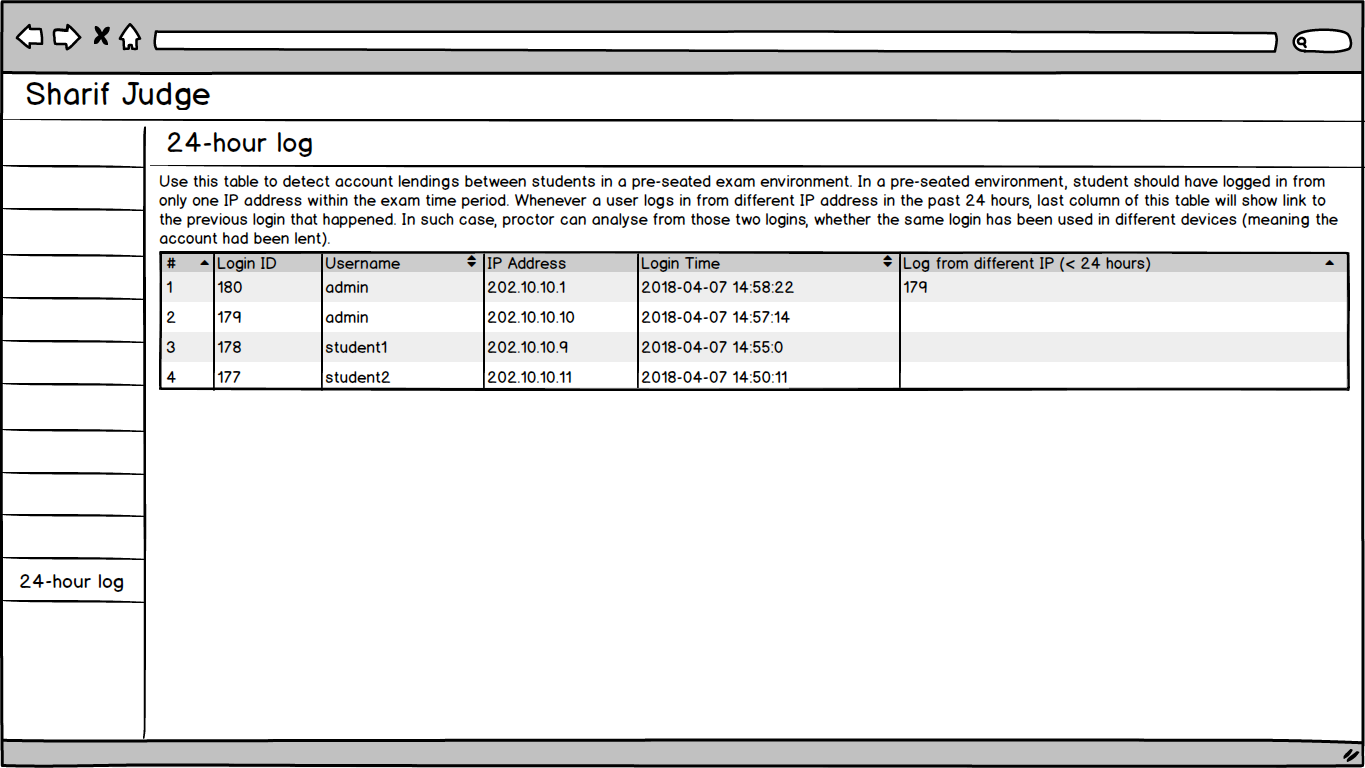
\includegraphics[width=1.0\textwidth]{mockuplogs}  
		\caption[Rancangan tampilan halaman \textit{logs}]{Rancangan tampilan halaman \textit{logs}} 
		\label{fig:mockuplogs} 
	\end{figure}

	\item \textit{Controller} \\
	\textit{Controller} untuk halaman \textit{logs} bernama \textit{Logs.php}. Pada \textit{controller Logs.php} terdapat beberapa fungsi. Tabel \ref{tab:f3logs} menunjukan perincian fungsi \textit{consturct\_\_} yang terdapat pada \textit{controller Logs.php}
	\begin{table}[H]
		\caption{Perincian fungsi \textit{consturct\_\_}}
		\label{tab:f3logs}
		\begin{tabular}{|c|p{11cm}|}
			\hline
			Nama \textit{Method} 	& 	\textit{consturct\_\_} 	\\
			\hline
			Parameter \textit{Input} & - \\
			\hline
			Parameter \textit{Output} &  - \\
			\hline
			Tabel yang berhubungan & - \\
			\hline
			Deskripsi	& membatasi pengguna yang dapat mengakses halaman \textit{logs}	 \\
			\hline
			Algoritma	& \begin{itemize}
				\item Mengecek \textit{session} pengguna yang akan mengakses halaman \textit{logs}.
				\item Jika \textit{session} tidak berstatus '\textit{logged\_in}, maka pengguna akan dialihkan ke halaman \textit{login}.
				\item Mengecek \textit{role} pengguna yang akan mengakses halaman \textit{logs}.
				\item Jika role pengguna bukan \textit{admin}, maka pengguna akan dialihkan ke halaman \textit{'404 Not Found'}.
			\end{itemize} \\
			\hline
		\end{tabular}
	\end{table}

	Tabel \ref{tab:f4logs} menunjukan perincian fungsi \textit{index} yang terdapat pada \textit{controller Logs.php}
	\begin{table}[H]
		\caption{Perincian fungsi \textit{index}}
		\label{tab:f4logs}
		\begin{tabular}{|c|p{11cm}|}
			\hline
			Nama \textit{Method} 	& 	\textit{index} 	\\
			\hline
			Parameter \textit{Input} & - \\
			\hline
			Parameter \textit{Output} &  - \\
			\hline
			Tabel yang berhubungan & \textit{shj\_logins} \\
			\hline
			Deskripsi	& Proses untuk memuat seluruh entri \textit{logs} pada halaman \textit{logs.twig}	 \\
			\hline
			Algoritma	& \begin{itemize}
				\item Memuat data \textit{logs} menggunakan fungsi \textit{get\_all\_logs} dari \textit{model Logs\_model.php}.
				\item Memproses data untuk tampilan \textit{logs.twig}.
			\end{itemize} \\
			\hline
		\end{tabular}
	\end{table}
\end{enumerate}

Selain menambahkan kelas \textit{model, view} dan \textit{controller}, terdapat perubahan kode pada kelas \textit{controller Login.php} dan \textit{config Install.php}. Perubahan kode di \textit{controller Login.php} untuk menyimpan data login pengguna ke dalam database. Listing \ref{lst:8} menunujukan hasil perubahan kode program yang dilakukan di \textit{controller Login.php}

\begin{lstlisting}[language=diff, caption=Perubahan kode program pada \textit{Login.php}, label=lst:8, basicstyle=\ttfamily, frame=single,
columns=fullflexible, keepspaces=true, breaklines=true]
@@ -53,6 +53,8 @@ class Login extends CI_Controller
$username = $this->input->post('username');
$password = $this->input->post('password');
if($this->user_model->validate_user($username, $password)){
+   $ip_adrress = $this->input->ip_address();
+
// setting the session and redirecting to dashboard:
$login_data = array(
	'username'  => $username,

@@ -60,6 +62,7 @@ class Login extends CI_Controller
);
	$this->session->set_userdata($login_data);
	$this->user_model->update_login_time($username);
+   	$this->logs_model->insert_to_logs($username,$ip_adrress);
	redirect('/');
}
else
\end{lstlisting}
~\\
Perubahan kode di \textit{config Install.php} untuk membuat tabel \textit{shj\_logins} pada \textit{database} saat penginstalan \textit{SharIF Judge}. Listing \ref{lst:9} menunjukan hasil perubahan kode program yang dilakukan di \textit{config Install.php}

\begin{lstlisting}[language=diff, caption=Perubahan kode program pada \textit{Install.php}, label=lst:9, basicstyle=\ttfamily, frame=single,
columns=fullflexible, keepspaces=true, breaklines=true]
@@ -249,7 +249,18 @@ class Install extends CI_Controller
if ( ! $this->dbforge->create_table('users', TRUE))
show_error("Error creating database table ".$this->db->dbprefix('users'));

-
+   // create table 'logins'
+   $fields = array(
+      'login_id'            => array('type' => 'INT', 'constraint' => 11, 'unsigned' => TRUE, 'auto_increment' => TRUE),
+      'username'                      => array('type' => 'VARCHAR', 'constraint' => 20),
+      'ip_address'          => array('type' => 'VARCHAR', 'constraint' => 15),
+      'timestamp'             => array('type' => 'TIMESTAMP'),
+      'last_24h_login_id'   => array('type' => 'INT', 'constraint' => 11, 'null' => TRUE),
+   );
+   $this->dbforge->add_field($fields);
+   $this->dbforge->add_key('login_id', TRUE); // PRIMARY KEY
+   if ( ! $this->dbforge->create_table('logins', TRUE))
+      show_error("Error creating database table ".$this->db->dbprefix('logins'));

// add admin user
$this->user_model->add_user(
\end{lstlisting}

\section{Menambahkan Parameter "\textit{Display Name}" pada Pendaftaran Peserta \textit{Sharif Judge}}
Untuk dapat menambahkan parameter "\textit{Display Name}" pada pendaftaran peserta \textit{Sharif Judge}, diperlukan beberapa perubahan kode program. Berikut rancangan algoritma yang dilakukan
\begin{enumerate}
	\item Menambahkan parameter "\textit{Display Name}" pada fungsi \textit{add\_user} yang terdapat di \textit{model User\_model.php}.
	\item Mengubah pemisah (\textit{separator}) antar parameter pada fungsi \textit{add\_user}. Pemisah antar parameter yang awalnya menggunakan spasi diubah menggunakan tanda koma.
	\item Menambahkan keterangan parameter "\textit{Display Name}" pada halaman \textit{add\_user.twig} dan  \textit{add\_user\_result.twig}.
	\item Menambahkan \textit{Display Name} untuk \textit{admin} pada proses \textit{install Sharif Judge}.
	%\item Mengubah urutan data yang digunakan pada fungsi pendaftaran peserta melalui \textit{email}.
	\item Menambahkan \textit{text field Display Name} pada halaman \textit{Register} \textit{(Open Public Registration}).
\end{enumerate}
Dari rancangan algoritma yang diterapkan, terdapat perubahan kode pada beberapa kelas. Beberapa kelas tersebut antara lain \textit{controller Install.php, controller Login.php, model User\_model.php, view add\_user.twig, view add\_user\_result.twig} dan \textit{view register.twig}.
~\\
Perubahan kode di \textit{Install.php} untuk menambahkan \textit{Display Name admin}. Listing \ref{lst:10} menunjukan hasil perubahan kode program yang dilakukan di \textit{Install.php}

\begin{lstlisting}[language=diff, caption=Perubahan kode program pada \textit{Install.php}, label=lst:10, basicstyle=\ttfamily, frame=single,
columns=fullflexible, keepspaces=true, breaklines=true]
@@ -255,6 +255,7 @@ class Install extends CI_Controller
	$this->user_model->add_user(
	$this->input->post('username'),
	$this->input->post('email'),
+   	'Admin',
	$this->input->post('password'),
	'admin'
);
\end{lstlisting}
~\\
Perubahan kode di halaman \textit{controller Login.php} untuk menerima \textit{input} dari \textit{text field Display Name} halaman \textit{register.twig}. Listing \ref{lst:11} menunjukan hasil perubahan kode program yang dilakukan di \textit{Login.php}

\begin{lstlisting}[language=diff, caption=Perubahan kode program pada \textit{Login.php}, label=lst:11, basicstyle=\ttfamily, frame=single,
columns=fullflexible, keepspaces=true, breaklines=true]
@@ -102,6 +102,7 @@ class Login extends CI_Controller
	$this->user_model->add_user(
	$this->input->post('username'),
	$this->input->post('email'),
+   	$this->input->post('displayname'),
	$this->input->post('password'),
	'student'
);
\end{lstlisting}
~\\
Perubahan kode di \textit{User\_model.php} untuk menambahkan parameter "\textit{Display Name}" dan mengubah pemisah antar parameter menggunakan tanda koma. Listing \ref{lst:12} menunjukan hasil perubahan kode program yang dilakukan di \textit{User\_model.php}

\begin{lstlisting}[language=diff, caption=Perubahan kode program pada \textit{User\_model.php}, label=lst:12, basicstyle=\ttfamily, frame=single,
columns=fullflexible, keepspaces=true, breaklines=true]
@@ -118,7 +118,7 @@ class User_model extends CI_Model
* @param $role
* @return bool|string
*/
-   public function add_user($username, $email, $password, $role)
+   public function add_user($username, $email, $display_name, $password, $role)
{
if ( ! $this->form_validation->alpha_numeric($username) )
return 'Username may only contain alpha-numeric characters.';

@@ -137,6 +137,7 @@ class User_model extends CI_Model
	$user=array(
	'username' => $username,
	'email' => $email,
+   	'display_name' => $display_name,
	'password' => $this->password_hash->HashPassword($password),
	'role' => $role
);

@@ -173,26 +174,26 @@ class User_model extends CI_Model
if (strlen($line) == 0 OR $line[0] == '#')
continue; //ignore comments and empty lines

-       $parts = preg_split('/\s+/', $line);
-   if (count($parts) != 4)
-   	continue; //ignore lines that not contain 4 parts
+       $parts = preg_split('/,+/', $line);
+   if (count($parts) != 5)
+       continue; //ignore lines that not contain 5 parts

-    if (strtolower(substr($parts[2], 0, 6)) == 'random')
+    if (strtolower(substr($parts[3], 0, 6)) == 'random')
{
// generate random password
-    $len = trim(substr($parts[2], 6), '[]');
+    $len = trim(substr($parts[3], 6), '[]');
	if (is_numeric($len)){
	$this->load->helper('string');
-   	$parts[2] = shj_random_password($len);
+       $parts[3] = shj_random_password($len);
	}
}

-   $result = $this->add_user($parts[0], $parts[1], $parts[2], $parts[3]);
+   $result = $this->add_user($parts[0], $parts[1], $parts[2], $parts[3], $parts[4]);

	if ($result === TRUE)
-   	array_push($users_ok, array($parts[0], $parts[1], $parts[2], $parts[3]));
+       array_push($users_ok, array($parts[0], $parts[1], $parts[2], $parts[3], $parts[4]));
	else
-       array_push($users_error, array($parts[0], $parts[1], $parts[2], $parts[3], $result));
+       array_push($users_error, array($parts[0], $parts[1], $parts[2], $parts[3], $parts[4], $result));

} // end of loop
\end{lstlisting}
~\\
Perubahan kode di halaman \textit{add\_user.twig} dan \textit{add\_user\_result.twig} untuk menambahkan keterangan parameter "\textit{Display Name}". Listing \ref{lst:13} menunjukan hasil perubahan kode program yang dilakukan di halaman \textit{add\_user.twig}. Listing \ref{lst:14} menunjukan hasil perubahan kode program yang dilakukan di halaman \textit{add\_user\_result.twig}

\begin{lstlisting}[language=diff, caption=Perubahan kode program pada halaman \textit{add\_user.twig}, label=lst:13, basicstyle=\ttfamily, frame=single,
columns=fullflexible, keepspaces=true, breaklines=true]
@@ -64,7 +64,7 @@
# Each line (except comments) represents a user.
# The syntax of each line is:
#
-   # USERNAME EMAIL PASSWORD ROLE
+   # USERNAME,EMAIL,DISPLAY-NAME,PASSWORD,ROLE
#
# Roles: admin head_instructor instructor student
# You can use RANDOM[n] for password to generate random n-digit password.
\end{lstlisting}
~\\

\begin{lstlisting}[language=diff, caption=Perubahan kode program pada halaman \textit{add\_user\_result.twig}, label=lst:14, basicstyle=\ttfamily, frame=single,
columns=fullflexible, keepspaces=true, breaklines=true]
@@ -7,7 +7,7 @@
<p class="shj_ok">These users added successfully:</p>
<ol>

-   <li>Usename: {{ item[0] }} Email: {{ item[1] }} Password: <code>{{ item[2] }}</code> Role: {{ item[3] }}</li>
+   <li>Usename: {{ item[0] }} Email: {{ item[1] }} Diplay Name: {{ item[2] }} Password: <code>{{ item[3] }}</code> Role: {{ item[4] }} </li>

</ol>

@@ -15,7 +15,7 @@
<p class="shj_error">Error adding these users:</p>
<ol>

-   <li>Usename: {{ item[0] }} Email: {{ item[1] }} Password: <code>{{ item[2] }}</code> Role: {{ item[3] }} ({{ item[4] }})</li>
+   <li>Usename: {{ item[0] }} Email: {{ item[1] }} Diplay Name: {{ item[2] }} Password: <code>{{ item[3] }}</code> Role: {{ item[4] }} ({{ item[5] }})</li>

</ol>
\end{lstlisting}
~\\
Perubahan kode di halaman \textit{register.twig} untuk menambahkan \textit{text field Display Name}. Listing \ref{lst:15} menunjukan hasil perubahan kode program yang dilakukan di halaman \textit{register.twig}
\begin{lstlisting}[language=diff, caption=Perubahan kode program pada halaman \textit{register.twig}, label=lst:15, basicstyle=\ttfamily, frame=single,
columns=fullflexible, keepspaces=true, breaklines=true]
@@ -32,6 +32,11 @@
<input id="form_email" type="email" autocomplete="off" name="email" required="required" class="sharif_input" value="{{ set_value('email') }}"/>
{{ form_error('email','<div class="shj_error">','</div>') }}
</p>
+      <p>
+         label for="form_displayname">Display Name</label><br/>
+         <input id="form_displayname" type="text" name="displayname" required="required" pattern="[A-Za-z\s]+" title="The Display Name field must be contain only alphabetical letters" class="sharif_input" value="{{ set_value('displayname') }}"/>
+         {{ form_error('form_displayname', '<div class="shj_error">', '</div>') }}
+      </p>
<p>
<label for="form_password">Password</label><br/>
<input id="form_password" type="password" name="password" required="required" pattern=".{6,200}" title="The Password field must be at least 6 characters in length" class="sharif_input"/>
\end{lstlisting}

\section{Menambahkan Fitur "\textit{Lock Student's Display Name}"}
\label{chap:lock}
Fitur "\textit{Lock Student's Display Name}" membutuhkan sebuah "\textit{key}" pada \textit{database}."\textit{Key}" tersebut berfungsi untuk menyimpan sebuah nilai. Nilai yang disimpan akan menentukan apakah para peserta dapat mengubah \textit{Display Name} atau tidak. "\textit{Key}" disimpan pada tabel \textit{shj\_settings} pada kolom \textit{shj\_key} dengan nama \textit{lock\_student\_display\_name}. \textit{lock\_student\_display\_name} memiliki nilai \textit{default shj\_value} = 0. Jika nilai dari \textit{lock\_student\_display\_name} = 1, maka para peserta tidak dapat mengubah \textit{Display Name}, sebaliknya jika bernilai 0, maka para peserta dapat mengubah \textit{Display Name}.

Rancangan algoritma yang digunakan untuk menambahkan fitur "\textit{Lock Student's Display Name}" yaitu
\begin{enumerate}
	\item Menambahkan \textit{shj\_key} dengan nama \textit{lock\_student\_display\_name} yang memiliki nilai \textit{shj\_value} = 0 pada tabel \textit{shj\_settings}.
	\item Menambahkan \textit{check box} pada halaman \textit{settings.twig} untuk mengaktifkan atau menonaktifkan fitur "\textit{Lock Student's Display Name}".
	\item Jika fitur "\textit{Lock Student's Display Name}" diaktifkan, maka \textit{text field Display Name} pada halaman \textit{profile.twig} akan dinonaktifkan (\textit{disabled}).
	\item Jika fitur "\textit{Lock Student's Display Name}" dinonaktifkan, maka \textit{text field Display Name} pada halaman \textit{profile.twig} akan kembali aktif.
	\item Menambahkan fungsi untuk mengecek kembali nilai dari \textit{lock\_student\_display\_name} pada saat peserta menyimpan perubahan yang dilakukan di halaman \textit{profile.twig}. Hal tersebut dilakukan untuk menangani para peserta yang "memaksa" agar dapat mengubah \textit{Display Name} dengan cara \textit{inspect element} lalu menghapus kode "\textit{disabled}" pada \textit{text field Display Name}.
\end{enumerate}

Dari rancangan algoritma yang diterapkan, terdapat perubahan kode pada beberapa kelas. Beberapa kelas tersebut antara lain \textit{controller Profile.php, controller Settings.php, model User\_model.php, view settings.twig}, \textit{view profile.twig} dan \textit{config Install.php}.
~\\
Perubahan  kode di \textit{Profile.php} untuk mengirimkan nilai '\textit{lock\_student\_display\_name}' ke halaman \textit{profile.twig}. Listing \ref{lst:16} menunjukan hasil perubahan kode program yang dilakukan di \textit{Profile.php}

\begin{lstlisting}[language=diff,caption=Perubahan kode program pada \textit{Profile.php}, label=lst:16, basicstyle=\ttfamily, frame=single,
columns=fullflexible, keepspaces=true, breaklines=true]
@@ -64,6 +64,7 @@ class Profile extends CI_Controller
	'display_name' => $user->display_name,
	'role' => $user->role,
	'form_status' => $this->form_status,
+   	'lock_student_display_name' => $this->settings_model->get_setting(lock_student_display_name),
	);

$this->twig->display('pages/profile.twig', $data);
\end{lstlisting}
~\\
Perubahan  kode di \textit{Settings.php} untuk menyimpan nilai dari \textit{check box} fitur "\textit{Lock Student's Display Name}" dari halaman \textit{settings.twig} ke \textit{database}. Listing \ref{lst:17} menunjukan hasil perubahan kode program yang dilakukan di \textit{Settings.php}

\begin{lstlisting}[language=diff, caption=Perubahan kode program pada \textit{Settings.php}, label=lst:17, basicstyle=\ttfamily, frame=single,
columns=fullflexible, keepspaces=true, breaklines=true]
@@ -113,9 +113,10 @@ class Settings extends CI_Controller
	'results_per_page_all' => $this->input->post('rpp_all'),
	'results_per_page_final' => $this->input->post('rpp_final'),
	'week_start' => $this->input->post('week_start'),
+   	'lock_student_display_name' => $this->input->post('lock_student_display_name')===NULL?0:1,
	)
);
\end{lstlisting}
~\\
Perubahan kode di \textit{User\_model.php} untuk mengecek apakah fitur "\textit{Lock Student's Display Name}" aktif atau tidak aktif. Listing \ref{lst:18} menunjukan hasil perubahan kode program yang dilakukan di \textit{User\_model.php}

\begin{lstlisting}[language=diff, caption=Perubahan kode program pada \textit{User\_model.php}, label=lst:18, basicstyle=\ttfamily, frame=single,
columns=fullflexible, keepspaces=true, breaklines=true]
@@ -404,9 +404,15 @@ class User_model extends CI_Model
return FALSE;
$the_user = $query->row();
$username = $the_user->username;
+
+   $display_name = $this->input->post('display_name');
+   $locked = $this->settings_model->get_setting(lock_student_display_name);
+   	if ($locked == 1) {
+          $display_name = $the_user->display_name;
+       }

	$user=array(
-   		'display_name' => $this->input->post('display_name'),
+      		'display_name' => $display_name,
		'email' => $this->input->post('email')
);
\end{lstlisting}
~\\
Perubahan kode di \textit{settings.twig} untuk menambahkan check box fitur "\textit{Lock Student's Display Name}". Listing \ref{lst:19} menunjukan hasil perubahan kode program yang dilakukan di halaman \textit{settings.twig}

\begin{lstlisting}[language=diff, caption=Perubahan kode program pada halaman \textit{settings.twig}, label=lst:19, basicstyle=\ttfamily, frame=single,
columns=fullflexible, keepspaces=true, breaklines=true]
@@ -114,6 +114,11 @@ $(document).ready(function(){
<label for="form_log">Log</label><br>
<span class="form_comment">Enable Log</span>
</p>
+   <p class="input_p">
+   		<input id="form_lock_student_display_name" type="checkbox" name="lock_student_display_name" value="1" {{ lock_student_display_name ? 'checked' }}/>
+   		<label for="form_lock_student_display_name">Lock Student's Display Name</label><br>
+           <span class="form_comment">Student's can't change their display name</span>
+   </p>
<p class="input_p">
	<label for="form_late_rule">Default Coefficient Rule</label>
	<span class="form_comment clear">PHP script without &lt;?php ?&gt; tags</span><br>
\end{lstlisting}
~\\
Perubahan kode di halaman \textit{profile.twig} untuk menentukan apakah \textit{text field Display Name} akan diaktifkan atau tidak. Listing \ref{lst:20} menunjukan hasil perubahan kode program yang dilakukan di halaman \textit{profile.twig}

\begin{lstlisting}[language=diff, caption=Perubahan kode program pada halaman \textit{profile.twig}, label=lst:20, basicstyle=\ttfamily, frame=single,
columns=fullflexible, keepspaces=true, breaklines=true]
@@ -28,7 +28,13 @@
</p>
<p class="input_p clear">
	<label for="form_name" class="short2">Name:</label>
-       <input id="form_name" type="text" name="display_name" class="sharif_input medium" value="{{ display_name }}"/>
+
+  
+  <input id="form_name" type="text" name="display_name" class="sharif_input medium" value="{{ display_name }}" disabled/>
+  
+  <input id="form_name" type="text" name="display_name" class="sharif_input medium" value="{{ display_name }}"/>
+  
+
	{{ form_error('display_name', '<div class="shj_error">', '</div>') }}
</p>
<p class="input_p clear">
\end{lstlisting}
~\\
Perubahan kode di \textit{config Install.php} untuk menambahkan atribut \linebreak \textit{lock\_student\_display\_name} pada tabel \textit{shj\_settings} di \textit{database} saat penginstalan \textit{SharIF Judge}. Listing \ref{lst:21} menunjukan perubahan kode di \textit{config Install.php}

\begin{lstlisting}[language=diff, caption=Perubahan kode program pada \textit{Install.php}, label=lst:21, basicstyle=\ttfamily, frame=single,
columns=fullflexible, keepspaces=true, breaklines=true]
@@ -220,6 +221,7 @@ class Install extends CI_Controller
array('shj_key' => 'results_per_page_all',   'shj_value' => '40'),
array('shj_key' => 'results_per_page_final', 'shj_value' => '80'),
array('shj_key' => 'week_start',             'shj_value' => '0'),
+   	array('shj_key' => 'lock_student_display_name',             'shj_value' => '1'),
));
if ( ! $result)
show_error("Error adding data to table ".$this->db->dbprefix('settings'));
\end{lstlisting}

\section{Menambahkan Fitur "\textit{Archived Assignment}"}
\label{chap:arc}
Fitur "\textit{Archived Assignment}" membutuhkan sebuah atribut baru pada \textit{database}. Atribut tersebut berfungsi untuk menyimpan sebuah nilai. Nilai yang disimpan akan menentukan apakah \textit{assignment} tersebut bersifat \textit{Archived Assignment} atau tidak. Atribut baru tersebut  ditambahkan pada tabel \textit{shj\_assignments} dengan nama \textit{archived\_assignment} yang menggunakan tipe data \textit{tinyint}. \textit{archived\_assignment} memiliki nilai \textit{default} = 0. Jika nilai dari \textit{archived\_assignment} = 1, maka \textit{assignment} tersebut merupakan sebuah \textit{archived\_assignment}, sebaliknya jika bernilai 0, maka \textit{assignment} tersebut merupakan \textit{assignment} biasa.

Rancangan algoritma yang digunakan untuk menambahkan fitur "\textit{Archived Assignment}" yaitu
\begin{enumerate}
	\item Menambahkan atribut baru dengan nama \textit{archived\_assignment} yang menggunakan tipe data \textit{tinyint}. Atribut baru tersebut ditambahkan pada tabel \textit{shj\_assignments}
	\item Menambahkan \textit{check box} pada halaman \textit{assignments.twig} untuk mengaktifkan atau menonaktifkan fitur "\textit{Archived Assignment}".
	\item Jika fitur "\textit{Archived Assignment}" diaktifkan, maka secara otomatis \textit{text field Start time} bernilai 1970-01-02 00:00:00, \textit{text field Finish Time} bernilai 2038-01-18 00:00:00 dan \textit{text field Extra Time} bernilai 0.
	\item \textit{Assignment} yang bersifat \textit{Archived Assignment} tidak muncul pada kalendar halaman \textit{dashboard}.
\end{enumerate}

Dari rancangan algoritma yang diterapkan, terdapat perubahan kode program pada beberapa kelas. Beberapa kelas tersebut antara lain \textit{model Assignment\_model.php, view add\_assignment.twig}, \textit{view dashboard.twig} dan \textit{config Install.php}.
~\\
Perubahan kode di \textit{Assignment\_model.php} untuk menyimpan nilai dari \textit{check box} fitur "\textit{Archived Assignment}" dari halaman \textit{add\_assignment.twig} ke \textit{database}. Listing \ref{lst:22} menunjukan hasil perubahan kode program yang dilakukan di \textit{Assignment\_model.php}

\begin{lstlisting}[language=diff, caption=Perubahan kode program pada \textit{Assignments\_model.php}, label=lst:22, basicstyle=\ttfamily, frame=single,
columns=fullflexible, keepspaces=true, breaklines=true]
@@ -38,6 +38,9 @@ class Assignment_model extends CI_Model
	{
	$extra_time *= $extra_item;
	}
+  
+   $archived_assignment = $archived_assignment = $this->input->post('archived_assignment')!==NULL ? 1 : 0;
+  
$assignment = array(
'id' => $id,
'name' => $this->input->post('assignment_name'),

@@ -51,7 +54,8 @@ class Assignment_model extends CI_Model
		'finish_time' => date('Y-m-d H:i:s', strtotime($this->input->post('finish_time'))),
		'extra_time' => $extra_time*60,
		'late_rule' => $this->input->post('late_rule'),
-       	'participants' => $this->input->post('participants')
+           'participants' => $this->input->post('participants'),
+           'archived_assignment' => $archived_assignment
	);
	if($edit)
	{
\end{lstlisting}
~\\
Perubahan kode di halaman \textit{add\_assignment.twig} untuk menambahkan \textit{check box} fitur "\textit{Archived Assignment}" dan  mengisi nilai \textit{text field Start time} menjadi 1970-01-02 00:00:00, \textit{text field Finish Time} menjadi 2038-01-18 00:00:00 serta \textit{text field Extra Time} menjadi 0. Listing \ref{lst:23} munujukan hasil perubahan kode program yang dilakukan di halaman \textit{add\_assignment.twig}

\begin{lstlisting}[language=diff, caption=Perubahan kode program pada halaman \textit{add\_assignment.twig}, label=lst:23, basicstyle=\ttfamily, frame=single, columns=fullflexible, keepspaces=true, breaklines=true]
@@ -39,6 +39,18 @@
			shj.num_of_problems++;
			$('#nop').attr('value', shj.num_of_problems);
		});
+    $("#form_a_archived_assignment").click(function(){
+                       if ($("#form_a_archived_assignment").is(':checked')) {
+        $("#start_time").val('1970-01-02 00:00:00');
+        $("#finish_time").val('2038-01-18 00:00:00');
+        $("#form_extra_time").val('0');
+      }
+      else{
+        $("#start_time").val('');
+        $("#finish_time").val('');
+        $("#form_extra_time").val('');
+      }
+               });
		$(document).on('click', '.delete_problem', function(){
		if (shj.num_of_problems==1) return;
		var row = $(this).parents('tr');
		
@@ -153,6 +165,12 @@
		<span class="form_comment space-left">Check this to show Java exceptions to users</span>
		{{ form_error('javaexceptions', '<div class="shj_error">', '</div>') }}
	</p>
+  <p class="input_p">
+            <input id="form_a_archived_assignment" type="checkbox" name="archived_assignment" value="1" {{ edit ? (edit_assignment.archived_assignment ? 'checked') : set_checkbox('archived_assignment', '1')|raw }} />
+            <label for="form_a_archived_assignment" class="default">Archived Assignment</label>
+            <span class="form_comment space-left">Check this to make an archived assignment</span>
+            {{ form_error('archived_assignment', '<div class="shj_error">', '</div>') }}
+   </p>
	<p class="input_p">
		<label for="form_late_rule">Coefficient rule (<a target="_blank" href="https://github.com/mjnaderi/Sharif-Judge/blob/docs/v1.4/add_assignment.md#coefficient-rule">?</a>)</label><br>
		<span class="form_comment medium clear" style="display: block;">PHP script without &lt;?php ?&gt; tags</span>
\end{lstlisting}
~\\
Perubahan kode di halaman \textit{dashboard.twig} untuk mengatur \textit{assignment} yang bersifat \textit{Archived Assignment} agar tidak muncul pada kalendar. Listing \ref{lst:24} menunjukan hasil perubahan kode program yang dilakukan di halaman \textit{dashboard.twig}

\begin{lstlisting}[language=diff, caption=Perubahan kode program pada halaman \textit{dashboard.twig}, label=lst:24, basicstyle=\ttfamily, frame=single,
columns=fullflexible, keepspaces=true, breaklines=true]
@@ -27,8 +27,13 @@ $(document).ready(function () {
	events: [
		
		
-       	{id:{{ assignment.id }},title:'{{ assignment.name|e('js') }}', start:'{{ assignment.start_time }}', end:' {{ assignment.finish_time }}',
-                               allDay:false,color:'{{ colors[(loop.index0)%colors|length] }}'}
+       	
+           	{id:{{ assignment.id }},title:'{{ assignment.name|e('js') }}', start:'{{ assignment.start_time }}', end:' {{ assignment.finish_time }}',
+               allDay:false,color:'{{ colors[(loop.index0)%colors|length] }}'}
+        	
+        	
+           	{}
+        	
		,
		
]
\end{lstlisting}
~\\
Perubahan kode di \textit{config Install.php} untuk menambahkan atribut \textit{archived\_assignment} pada tabel \textit{shj\_assignments} di \textit{database} saat penginstalan \textit{SharIF Judge}. Listing \ref{lst:25} menunjukan hasil perubahan kode di \textit{config Install.php}

\begin{lstlisting}[language=diff, caption=Perubahan kode program pada \textit{Install.php}, label=lst:25, basicstyle=\ttfamily, frame=single,
columns=fullflexible, keepspaces=true, breaklines=true]
@@ -105,6 +105,7 @@ class Install extends CI_Controller
	'late_rule'     => array('type' => 'TEXT'),
	'participants'  => array('type' => 'TEXT', 'default' => ''),
	'moss_update'   => array('type' => 'VARCHAR', 'constraint' => 30, 'default' => 'Never'),
+   	'archived_assignment'    => array('type' => 'TINYINT', 'constraint' => 1),
);
$this->dbforge->add_field($fields);
$this->dbforge->add_key('id', TRUE); // PRIMARY KEY
\end{lstlisting}

\section{Menambahkan Halaman \textit{Hall of Fame}}
Halaman \textit{Hall of Fame} tidak membutuhkan atribut atau tabel baru pada \textit{database} namun perlu ditambahkan \textit{model, view} dan \textit{controller}.

\begin{enumerate}
	\item \textit{Model} \\
	\textit{Model} untuk halaman \textit{Hall of Fame} bernama \textit{Hof\_model.php}. Pada \textit{model Hof\_model.php} terdapat beberapa fungsi. Tabel \ref{tab:f1hof} menunjukan perincian fungsi \textit{get\_all\_final\_submission} yang terdapat pada \textit{Hof\_model.php}
	\begin{table}[H]
		\caption{Perincian fungsi \textit{get\_all\_final\_submission}}
		\label{tab:f1hof}
		\begin{tabular}{|c|p{11cm}|}
			\hline
			Nama \textit{Method} 	& 	\textit{get\_all\_final\_submission} 	\\
			\hline
			Parameter \textit{Input} & - \\
			\hline
			Parameter \textit{Output} & semua entri nilai submissions yang telah dijumlahkan \\
			\hline
			Tabel yang berhubungan & \textit{shj\_submissions} \\
			\hline
			Deskripsi	& Proses untuk mengembalikan semua entri nilai submission yang telah djumlahkan pada tabel \textit{shj\_submissions} \\
			\hline
			Algoritma	& \begin{itemize}
				\item Menghitung dan menjumlahkan nilai seluruh problem pada setiap assignment peserta tertentu dengan menggunakan rumus perhitungan nilai dari \textit{Controller Submissions.php}. Rumus yang digunakan adalah \textit{SCORE = pre\_score * coefficient / 10000}.
				\item Menjumlahkan seluruh nilai assignment setiap peserta yang tidak bersifat "\textit{Upload Only}". Nilai yang telah dijumlahkan akan disimpan sebagai total skor.
				\item Mengurutkan total skor dari yang paling besar.
				\item Mengembalikan seluruh entri yang telah dijumlahkan dalam bentuk \textit{array}.
			\end{itemize} \\
			\hline
		\end{tabular}
	\end{table}
	
	Tabel \ref{tab:f2hof} menunjukan perincian fungsi \textit{get\_all\_user\_assignments} yang terdapat pada \linebreak \textit{Hof\_model.php}
	\begin{table}[H]
		\caption{Perincian fungsi \textit{get\_all\_user\_assignments}}
		\label{tab:f2hof}
		\begin{tabular}{|c|p{11cm}|}
			\hline
			Nama \textit{Method} 	& 	\textit{get\_all\_user\_assignments} 	\\
			\hline
			Parameter \textit{Input} & \textit{\$username} \\
			\hline
			Parameter \textit{Output} &  mengembalikan seluruh \textit{details} dari \textit{assignment} pengguna tertentu\\
			\hline
			Tabel yang berhubungan & \textit{shj\_submissions} \\
			\hline
			Deskripsi	& Proses untuk mengembalikan \textit{details assignment} pengguna tertentu. \textit{Details} berisikan nama \textit{assignment}, nama \textit{problem} dan skor \\
			\hline
			Algoritma	& \begin{itemize}
				\item Menyimpan nama \textit{assignment}, nama \textit{problem} dan skor setiap \textit{problem} dari sebuah \textit{assignment} pengguna tertentu.
				\item Mengembalikan \textit{details} di atas dalam bentuk \textit{array}.
			\end{itemize} \\
			\hline
		\end{tabular}
	\end{table}
	
	\item \textit{View} \\
	\textit{View} untuk halaman \textit{Hall of Fame} bernama \textit{halloffame.twig}. Menu halaman \textit{Hall of Fame} terletak di bawah menu \textit{Scoreboard}. Pada halaman ini juga berlaku sistem rangking sehingga nama para peserta yang muncul diurutkan bedasarkan total skor. Jika total skor yang dimiliki peserta memiliki nilai yang sama dengan peserta lainnya, maka peserta tersebut memiliki rangking yang sama dengan peserta lainnya. Gambar \ref{fig:mockuphof} menunjukan rancangan tampilan halaman \textit{Hall of Fame}. Gambar \ref{fig:mockuphofdetail} menunjukan rancangan tampilan \textit{detail} dari \textit{Hall of Fame}. 
	
	\begin{figure}[H]
		\centering  
		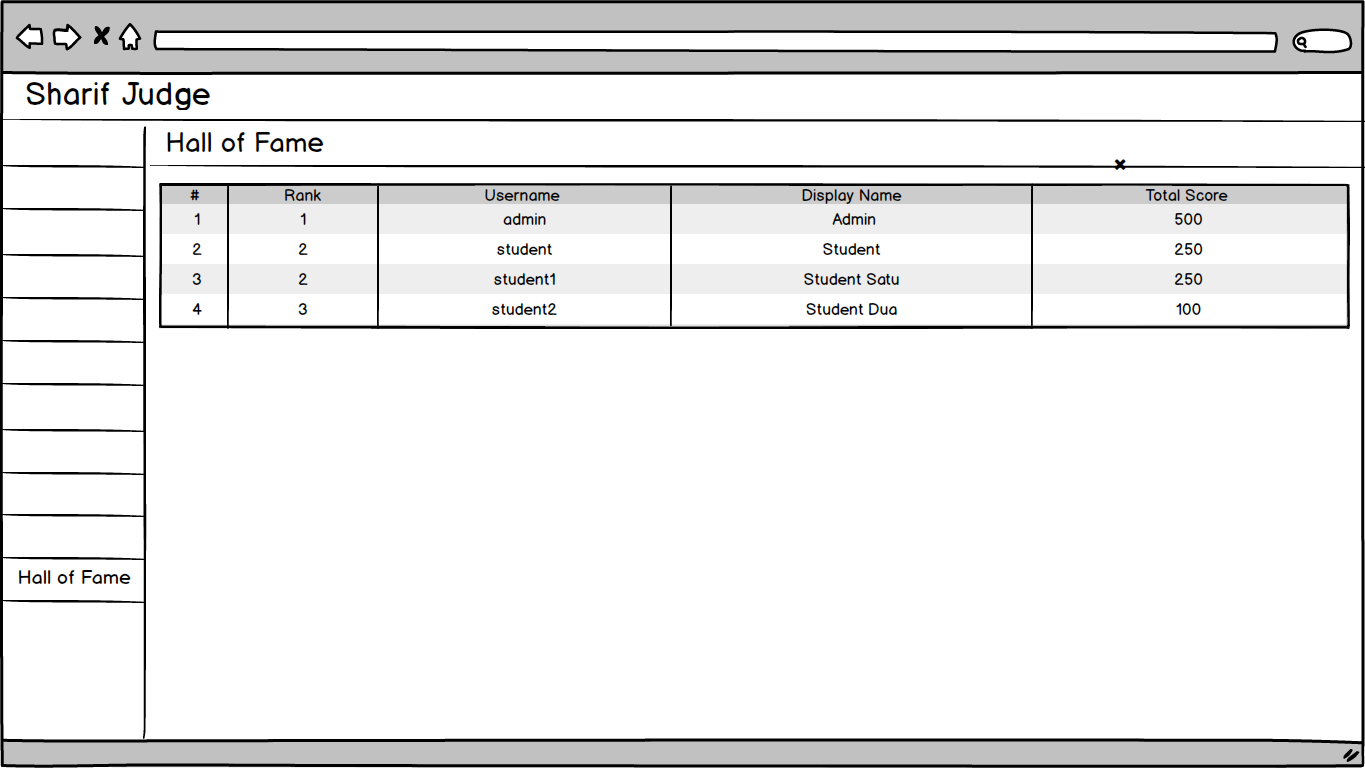
\includegraphics[width=1.0\textwidth]{mockuphof}  
		\caption[Rancangan tampilan halaman \textit{Hall of Fame}]{Rancangan tampilan halaman \textit{Hall of Fame}} 
		\label{fig:mockuphof} 
	\end{figure}

	\begin{figure}[H]
		\centering  
		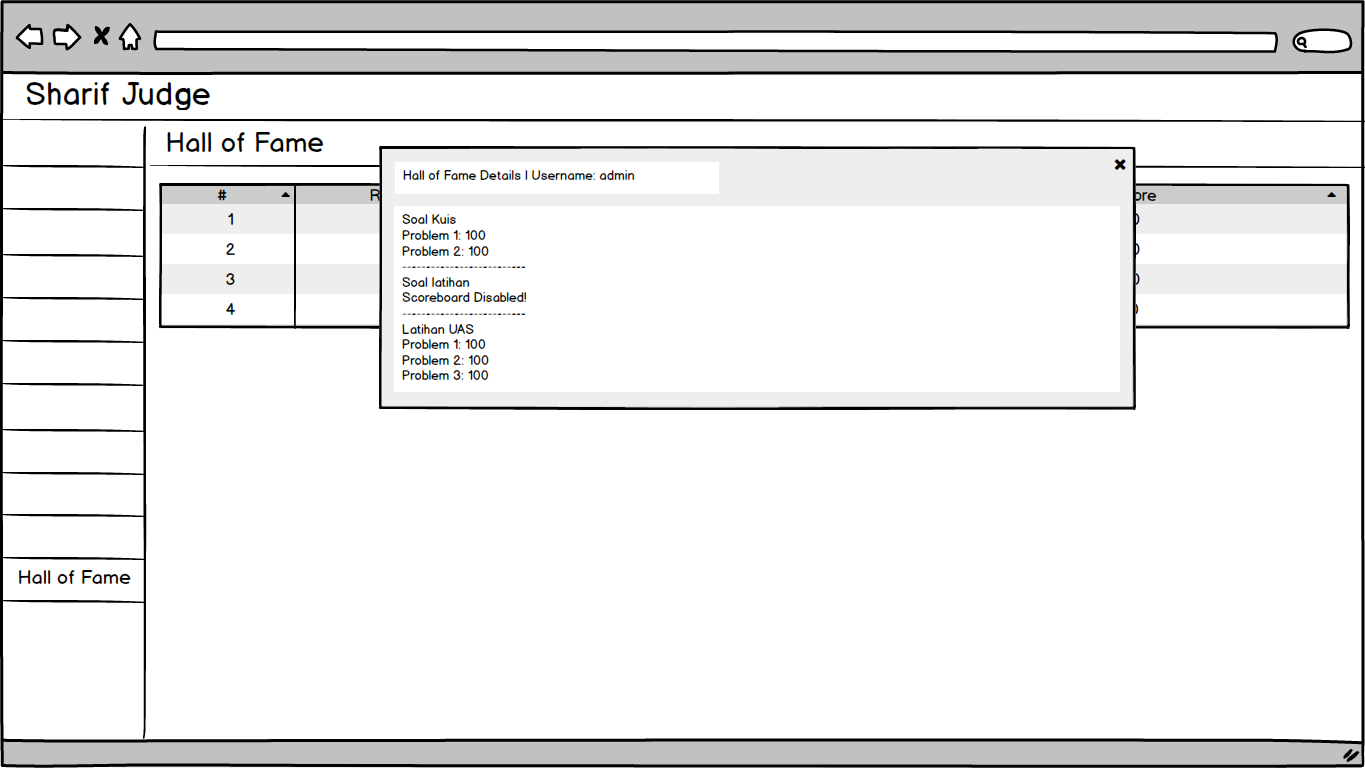
\includegraphics[width=1.0\textwidth]{mockuphofdetail}  
		\caption[Rancangan tampilan \textit{details} \textit{Hall of Fame} peserta tertentu]{Rancangan tampilan \textit{details} \textit{Hall of Fame} peserta tertentu} 
		\label{fig:mockuphofdetail} 
	\end{figure}
	
	\item \textit{Controller} \\
	\textit{Controller} untuk halaman \textit{Hall of Fame} bernama \textit{Halloffame.php}. Pada \textit{controller Halloffame.php} terdapat beberapa fungsi. Tabel \ref{tab:f3hof} menunjukan perincian fungsi \textit{consturct\_\_} yang terdapat pada \textit{Halloffame.php}
	\begin{table}[H]
		\caption{Perincian fungsi \textit{consturct\_\_}}
		\label{tab:f3hof}
		\begin{tabular}{|c|p{11cm}|}
			\hline
			Nama \textit{Method} 	& 	\textit{consturct\_\_} 	\\
			\hline
			Parameter \textit{Input} & - \\
			\hline
			Parameter \textit{Output} &  - \\
			\hline
			Tabel yang berhubungan & - \\
			\hline
			Deskripsi	& membatasi pengguna yang dapat mengakses halaman \textit{Hall of Fame}	 \\
			\hline
			Algoritma	& \begin{itemize}
				\item mengecek \textit{session} pengguna yang akan mengakses halaman \textit{Hall of Fame}.
				\item Jika \textit{session} tidak berstatus '\textit{logged\_in}, maka pengguna akan dialihkan ke halaman \textit{login}.
				\item Memuat \textit{model Hof\_model.php}.
			\end{itemize} \\
			\hline
		\end{tabular}
	\end{table}
	
	Tabel \ref{tab:f4hof} menunjukan perincian fungsi \textit{index} yang terdapat pada \textit{Halloffame.php}
	\begin{table}[H]
		\caption{Perincian fungsi \textit{index}}
		\label{tab:f4hof}
		\begin{tabular}{|c|p{11cm}|}
			\hline
			Nama \textit{Method} 	& 	\textit{index} 	\\
			\hline
			Parameter \textit{Input} & - \\
			\hline
			Parameter \textit{Output} &  - \\
			\hline
			Tabel yang berhubungan & \textit{shj\_submissions} \\
			\hline
			Deskripsi	& Proses untuk memuat seluruh entri \textit{submissions} yang telah dijumlahkan pada halaman \textit{halloffame.twig}	 \\
			\hline
			Algoritma	& \begin{itemize}
				\item Memuat data \textit{Hall of Fame} menggunakan fungsi \textit{get\_all\_final\_submission} dari \textit{model Hof\_model.php}.
				\item Memproses data untuk tampilan \textit{halloffame.twig}.
			\end{itemize} \\
			\hline
		\end{tabular}
	\end{table}
	
	Tabel \ref{tab:f5hof} menunjukan perincian fungsi \textit{hof\_details} yang terdapat pada \textit{Halloffame.php}
	\begin{table}[H]
		\caption{Perincian fungsi \textit{hof\_details}}
		\label{tab:f5hof}
		\begin{tabular}{|c|p{11cm}|}
			\hline
			Nama \textit{Method} 	& 	\textit{hof\_details} 	\\
			\hline
			Parameter \textit{Input} & - \\
			\hline
			Parameter \textit{Output} &  - \\
			\hline
			Tabel yang berhubungan & \textit{shj\_submissions} \\
			\hline
			Deskripsi	& Proses untuk memuat details \textit{submissions} pada halaman \textit{halloffame.twig}	 \\
			\hline
			Algoritma	& \begin{itemize}
				\item Memuat \textit{details} \textit{Hall of Fame} peserta tertentu menggunakan fungsi \textit{get\_all\_user\_assignments} dari \textit{model Hof\_model.php}.
				\item Memproses data untuk tampilan \textit{details} \textit{Hall of Fame} dari peserta tertentu pada halaman \textit{halloffame.twig}.
			\end{itemize} \\
			\hline
		\end{tabular}
	\end{table}
\end{enumerate}

Selain menambahkan kelas \textit{model, view} dan \textit{controller}, terdapat penambahan fungsi pada \textit{file shj\_functions.js} yang terletak di \path{Sharif-Judge\assets\js}. Penambahan fungsi tersebut berguna untuk meminta \textit{details} dari Hall of Fame peserta tertentu menggunakan fungsi hof\_details pada \textit{controller Halloffame.php} lalu menampilkannya. Hasil penamabahan dan perubahan kode program yang dilakukan di \textit{shj\_functions.js} dapat dilihat di \hyperref[lamp:kodeprogramshjfunc]{Lampiran C}

\section{Integrasi \textit{Login} ke \textit{Server RADIUS}}
\textit{Sharif Judge} memerlukan \textit{library} baru agar dapat mengintegrasikan \textit{login} ke \textit{server RADIUS}. \textit{Library} yang digunakan adalah \textit{Dapphp/Radius}. \textit{Dapphp/Radius} adalah klien \textit{RADIUS PHP} untuk mengautentikasi pengguna terhadap \textit{server RADIUS}. Cara yang disarankan untuk menginstal \textit{Dapphp/Radius} adalah menggunakan \textit{Composer}. Jika \textit{Composer} telah terinstall, maka jalankan perintah "\textit{composer require dapphp/radius}" atau tambahkan "\textit{dapphp/radius}" pada file \textit{composer.json} bagian "\textit{section}"~\cite{drew:16:radius}.

Rancangan algoritma yang digunakan untuk menambahkan mengintegrasikan \textit{login} ke \textit{server RADIUS} yaitu
\begin{enumerate}
	\item Menginstall \textit{Composer} pada perangkat lunak \textit{Sharif Judge}.
	\item Menambahkan \textit{library Dapphp/Radius} menggunakan \textit{Composer}.
	\item Membuat \textit{file secrets.php} pada direktori \path{Sharif-Judge\application\config} untuk menyimpan configurasi alamat \textit{server RADIUS}.
	\item Mengintegrasikan \textit{login} pengguna \textit{Sharif Judge} ke \textit{server RADIUS}.
\end{enumerate}

Dari rancangan algoritma yang diterapkan, terdapat perubahan kode pada kelas \textit{model User\_model.php}.
~\\
Perubahan kode di model \textit{User\_model.php} untuk memanggil \textit{library Dapphp/Radius} dan mengintegrasikan \textit{login} pengguna \textit{Sharif Judge} ke \textit{server RADIUS}. Listing \ref{lst:26} menunjukan hasil perubahan kode program yang dilakukan di \textit{User\_model.php}

\begin{lstlisting}[language=diff, caption=Perubahan kode program pada \textit{User\_model.php}, label=lst:26, basicstyle=\ttfamily, frame=single,
columns=fullflexible, keepspaces=true, breaklines=true]
@@ -5,6 +5,7 @@
* @author Mohammad Javad Naderi <mjnaderi@gmail.com>
*/
defined('BASEPATH') OR exit('No direct script access allowed');
+   use Dapphp\Radius\Radius;

class User_model extends CI_Model
{

@@ -330,6 +331,15 @@ class User_model extends CI_Model
		return FALSE;
	if ($this->password_hash->CheckPassword($password, $query->row()->password))
		return TRUE;
+  
+   	$this->load->config('secrets');
+       if($this->config->item('shj_authenticate') == 'radius') {
+       	$client = new Radius();
+           $client->setServer($this->config->item('shj_radius')['server']) // RADIUS server address
+                  ->setSecret($this->config->item('shj_radius')['secret']);
+           if($client->accessRequest($username, $password))
+           	return TRUE;
+       }
	return FALSE;
}
\end{lstlisting}

Kode program file secrets.php dapat dilihat di \hyperref[lamp:kodeprogramsecrets]{Lampiran D}.

\section{Branding Teknik Informatika}
Branding Teknik Informatika dilakukan dengan cara mengubah seluruh logo dan ikon \textit{Sharif Judge} menggunakan logo dan ikon Teknik Informatika. Gambar \ref{fig:logosmall} menunjukan logo dan ikon Teknik Informatika yang digunakan. Gambar \ref{fig:banner} \textit{banner Sharif Judge} yang digunakan.

\begin{figure}[H]
	\centering  
	
\includegraphics[scale=1]{logosmall}  
	\caption[Logo dan Ikon]{Logo dan Ikon} 
	\label{fig:logosmall} 
\end{figure} 

\begin{figure}[H]
	\centering  
	
\includegraphics[scale=1]{banner}  
	\caption[\textit{Banner Sharif Judge}]{\textit{Banner Sharif Judge}} 
	\label{fig:banner} 
\end{figure} 

Agar dapat menggunakan logo dan ikon Teknik Informatika dibutuhkan penggantian beberapa file. Beberapa \textit{file} tersebut antara lain \textit{banner.png, favicon.ico} dan \textit{logo\_small.png} yang terdapat pada \path{Sharif-Judge\assets\images}. Penggantian beberapa \textit{file} tersebut mencakup \textit{banner} pada halaman \textit{login}, icon pada \textit{title bar} dan \textit{top bar}.

Langkah-langkah yang dilakukan untuk proses branding Teknik Informatika adalah
\begin{enumerate}
	\item Menggunakan logo dan ikon Teknik Informatika pada \textit{Sharif Judge}.
	\item Mengubah nama \textit{Sharif Judge} menjadi SharIF Judge.
	\item Mengubah link dokumentasi \textit{Github Sharif Judge} menjadi \path{https://github.com/ftisunpar/Sharif-Judge}.
\end{enumerate}